%%%%%%%%%%%%%%%%%%%%%%%%%%%%%%%%%%%%%%%%%%%%%%%%%%%%%%%%%%%%%%%%%%%%%%%%%%%%%%%
% ICML 2027 submission
%%%%%%%%%%%%%%%%%%%%%%%%%%%%%%%%%%%%%%%%%%%%%%%%%%%%%%%%%%%%%%%%%%%%%%%%%%%%%%%
\documentclass{article}

\usepackage{microtype}
\usepackage{graphicx}
\usepackage{subfigure}
\usepackage{booktabs}
\usepackage{hyperref}
\newcommand{\theHalgorithm}{\arabic{algorithm}}

% Blind submission for review:
\usepackage{icml2027}
% Camera ready instead uses:
% \usepackage[accepted]{icml2027}

\usepackage{amsmath}
\usepackage{amssymb}
\usepackage{mathtools}
\usepackage{amsthm}
\usepackage{pgfplots}
\pgfplotsset{compat=1.17}
\usepackage[capitalize,noabbrev]{cleveref}

\theoremstyle{plain}
\newtheorem{theorem}{Theorem}[section]
\newtheorem{proposition}[theorem]{Proposition}
\newtheorem{lemma}[theorem]{Lemma}
\newtheorem{corollary}[theorem]{Corollary}
\theoremstyle{definition}
\newtheorem{definition}[theorem]{Definition}

\newcommand{\yhat}{\hat{y}}
\newcommand{\Exp}{\mathbb{E}}
\newcommand{\Real}{\mathbb{R}}
\newcommand{\He}{\mathrm{He}}
\newcommand{\Normal}{\mathcal{N}}

\icmltitlerunning{The Misspecification Gap in Model-Guided Design}

\begin{document}

\twocolumn[
\icmltitle{The Misspecification Gap in Model-Guided Design}

\begin{icmlauthorlist}
\icmlauthor{Anonymous Authors}{anon}
\end{icmlauthorlist}

\icmlaffiliation{anon}{Anonymous Institution}
\icmlcorrespondingauthor{Anonymous Authors}{anon@example.com}

\icmlkeywords{model misspecification, model-guided design, protein fitness, calibration}

\vskip 0.3in
]

\printAffiliationsAndNotice{}

\begin{abstract}
Model-guided design trains a surrogate on measured data, ranks a large candidate
library by predicted value, and sends the top $K$ candidates to the next round of
experiments. The predicted value of that batch is routinely treated as a forecast of
what the batch will deliver, and it is routinely too high. We show that this gap is
not a consequence of selection as such. A surrogate that reports the conditional mean
of fitness given its own score is unbiased on any selected subset, however extreme the
selection, by the tower property. The gap instead measures how far the reported score
is from that conditional mean, so it is a misspecification gap, and we derive it in
closed form. Writing the fitness distribution as a monotone transform $G$ of a standard
Gaussian variable, the gap depends only on the nonlinear Hermite components of $G$, so
it vanishes exactly when fitness is Gaussian and persists at full strength when the
surrogate ranks candidates perfectly. The theory predicts that the gap grows as the
upper tail of the fitness distribution is compressed and reverses sign when that tail
is long. On $217$ deep mutational scanning assays we find that $93\%$ of assays
overpromise, that the gap holds near $23\%$ of the achievable gain across surrogate
accuracies from $0.5$ to $0.9$, and that a one-line statistic of the fitness
distribution predicts the gap and its reversal, with the fraction of underpromising
assays rising from $0\%$ to $42\%$ as the tail lengthens. The same gap appears under
protein language model surrogates and in superconductors, small molecules, and
antimicrobial peptides. The diagnosis is
constructive: estimating the conditional mean by isotonic regression on held-out data
cuts the mean absolute gap from $0.245$ to $0.100$ and the median gap from $0.166$ to
$0.057$, winning on $76\%$ of assay and budget combinations, while leaving the selected
batch and therefore the realized gain untouched.
\end{abstract}

\section{Introduction}
\label{sec:intro}

A protein engineering campaign rarely measures every candidate it cares about. A
library of $10^4$ to $10^6$ variants is far larger than an assay budget of a few
hundred, so practitioners train a surrogate model on whatever measurements exist,
score the full library with it, and carry the highest scoring candidates into the next
experimental round. This loop, usually called machine learning guided directed
evolution, now underlies a large share of published protein design work, and the same
pattern appears in small molecule screening and materials discovery.

Two numbers govern how such a campaign is planned. The first is the accuracy of the
surrogate, almost always reported as a rank correlation between predicted and measured
fitness on held-out data. The second is the predicted value of the selected batch,
which tells the team what the round is expected to deliver and therefore whether it is
worth running. Benchmarks have concentrated almost entirely on the first number.
Leaderboards rank models by held-out correlation, and a model that scores well is taken
to be a model worth deploying.

The second number has received far less scrutiny, and it is the one that sets
expectations. If a surrogate reports that its chosen batch will improve on the
wild type by a given margin, and the batch in fact delivers less, then every downstream
decision built on that margin is distorted. The team overestimates the value of the
round, underestimates how many rounds are needed, and may conclude that an assay is
noisy when the model was simply optimistic. A natural assumption is that this gap is a
symptom of a weak surrogate and that it closes as models improve.

We show that this assumption is wrong, and that the gap has a specific and predictable
structure. It is tempting to attribute the gap to selection itself, on the reasoning
that choosing the highest scoring candidates conditions on a region where prediction
error happens to be positive. That reasoning does not survive contact with the tower
property. If the reported score is the conditional mean of fitness given the
surrogate's own output, then the expected gap on any selected subset is exactly zero,
no matter how extreme the selection. Selection alone therefore cannot produce a gap.

What produces it is the discrepancy between the quantity a team reports and the
conditional mean it is taken to be. A surrogate is fit to predict
fitness from features, so its output estimates the conditional mean of fitness given
those features, which is not the conditional mean given the output itself unless the
fit is exact. Tuning and benchmarking for rank accuracy does nothing to close that
difference, so the reported score carries the right ordering and the wrong magnitude. The gap measures exactly that discrepancy, which is why we
call it a misspecification gap. Its size is governed by how far the fitness
distribution departs from Gaussian in its upper tail, so it is a property of the assay
and of the form of the score rather than a deficiency of the fit, and improving rank
accuracy does not remove it.

Reading the gap this way turns a diagnosis into a remedy. Because the gap is the
distance between the reported score and a conditional mean, estimating that conditional
mean closes it. Any strictly increasing map from score to forecast leaves the ranking,
and therefore the selected batch and the realized gain, exactly as they were, so the
forecast can be repaired without disturbing the design. We estimate the conditional
mean by isotonic regression on held-out data and recover most of the gap. Separating
the quality of the forecast from the quality of the selection is what makes this
possible, and our tail statistic predicts in advance, from the measured fitness values
alone and before any model is fit, how large the uncorrected gap will be.

Our contributions are as follows.

\begin{itemize}
\item We separate selection from misspecification. A conditional-mean forecast is
unbiased under any score-based selection (\cref{prop:tower}), which is the
auto-calibration property and not new, and on that premise the gap of a calibrated
score has a closed form (\cref{thm:main}). It is exactly $0$ at every accuracy when fitness is Gaussian
(\cref{cor:gaussian}) and tends to a nonzero constant as accuracy approaches a perfect
ranking (\cref{cor:saturation}).
\item We define a scale-free index of upper-tail compression, computable before any
model is fit, that predicts the size and sign of the gap and forecasts it on held-out
assays better than trusting the surrogate.
\item We quantify the gap on $217$ deep mutational scanning assays. It persists across
surrogate families, grows when language-model scores raise accuracy, is absent for a
random forest, whose output is an average, and appears in materials, small-molecule,
and peptide data.
\item We show that isotonic estimation of the conditional mean removes most of the gap
without changing the selected batch, where binned, Tweedie, and conformal corrections
do not, and that rules which rescale or diversify the selection fail to recover gain.
\end{itemize}

The rest of the paper is organized as follows. \Cref{sec:related} reviews work on
fitness prediction benchmarks, selection bias, and model-guided design.
\Cref{sec:method} sets up the selection problem, states the main result and its
corollaries, and defines the tail-compression index. \Cref{sec:setup} describes the
assays, the surrogate, and the evaluation protocol. \Cref{sec:results} reports the
measured gap, the tests of the theory, the correction rules, and the results for other
surrogates and other domains.
\Cref{sec:discussion} discusses what the results change for practice, and
\Cref{sec:conclusion} concludes.

\section{Related Work}
\label{sec:related}

\paragraph{Benchmarks for protein fitness prediction.}
Deep mutational scanning measures the functional effect of thousands of single amino
acid substitutions in one experiment \citep{fowler2014deep}, and the accumulation of
these datasets made systematic benchmarking possible. ProteinGym collects $217$
substitution assays and reports rank correlation, top-$K$ recall, and normalized
discounted cumulative gain \citep{notin2023proteingym}.
Models evaluated on it range from alignment-based methods \citep{hopf2017mutation,
frazer2021disease} to protein language models trained on unaligned sequences
\citep{rives2021biological, lin2023evolutionary, elnaggar2021prottrans,
madani2023large}, hybrids that retrieve homologs at inference time
\citep{notin2022tranception}, and structure-aware scorers \citep{meier2021language,
cheng2023accurate}. Accuracy on these benchmarks has risen steadily, which makes the
question of what it buys a design campaign more pressing rather than less.

\paragraph{From ranking quality to design outcomes.}
Several authors have questioned whether leaderboard position transfers to design.
\citet{notin2023proteingym} note that averaging correlations across proteins can
mislead because assays differ in dynamic range and in how much of the fitness scale is
biologically meaningful. \citet{wang2026goodfilters} compare $97$ models across the
same $217$ assays and find that the model ranked best by correlation is only weakly
predictive of which model is best at sites where models disagree, and that correlation
and discounted gain select different winners in every assay category. That work is
diagnostic and compares models to each other. We ask a different question, namely how
far a single surrogate's own forecast departs from what its chosen batch delivers, and
we give the departure in closed form.

\paragraph{Model-guided design loops.}
Machine learning guided directed evolution trains a surrogate on measured variants and
proposes the next batch from its predictions \citep{yang2019machine, wu2019machine,
biswas2021low}. Such systems differ in how they balance exploitation against exploration
\citep{hie2022adaptive, brookes2019conditioning, stanton2022accelerating}, construct
libraries \citep{sinai2020adalead}, and handle batches
\citep{angermueller2020modelbased}. The same loop is studied without the wet lab as
offline model-based optimization, where a fixed dataset must be turned into designs and
the surrogate is known to be unreliable away from the data it was fit on
\citep{trabucco2021coms, fannjiang2020autofocused}, and where a standard benchmark now
exists \citep{trabucco2022designbench}. Those methods act on the ordering, by holding the surrogate
down on out-of-distribution inputs or by refitting it as the search moves; the gap we
study survives any such change because it concerns the number attached to the batch
rather than the batch itself. A recurring observation is that candidates
predicted to be strong can differ substantially from those that measure strongly, and
that quantifying uncertainty for designed candidates has to account for the feedback
loop that produced them \citep{hsu2022learning, fannjiang2022conformal}. Our results explain part of that
pattern and show that it does not disappear as the surrogate improves.

\paragraph{Selection bias and the winner's curse.}
That estimates conditioned on being extreme are biased is classical. In decision
analysis it is the optimizer's curse: ranking alternatives by unbiased value estimates
and acting on the best leaves one disappointed on average, and the remedy is to replace
each estimate by its posterior mean \citep{smith2006optimizer}. \Cref{prop:tower} is
that remedy stated for model-guided design, and we present it as the premise that makes
the rest of the analysis precise rather than as a new result.
In genetics the effect is known as the winner's curse: effect sizes for variants
selected by significance are inflated, and a literature of corrections has grown around
it \citep{goring2001large, zollner2007overcoming, zhong2008bias, palmer2017statistical,
forde2023review}. Related corrections appear in expression quantitative trait analysis
\citep{huang2018bootstrapqtl} and in Mendelian randomization
\citep{sadreev2021empirical}. Directed evolution has its own version, where variant
scores estimated from sequencing counts are biased upward for top ranked variants
\citep{nemoto2023acides}. The empirical Bayes remedy is Tweedie's formula, which
corrects a selected estimate by the local derivative of the log marginal density and
which \citet{efron2011tweedie} develops precisely as a treatment for selection bias.
Selective inference provides general machinery for
conditioning on a selection event \citep{benjamini2005false, taylor2015statistical,
tibshirani2016exact, fithian2014optimal}. These treatments share a Gaussian or
exponential-family assumption on the quantity being selected. The contribution here is
to show that in model-guided design the bias is controlled not by the noise level but by
the shape of the fitness distribution, so that it survives even an arbitrarily accurate
ranking, and to identify the distributional feature that governs its magnitude and its
sign.

\paragraph{Calibration.}
Post hoc calibration adjusts predicted values so that they match observed outcomes on
held-out data, through isotonic regression \citep{zadrozny2002transforming}, Platt
scaling \citep{platt1999probabilistic}, temperature scaling
\citep{guo2017calibration}, or conformal prediction \citep{vovk2005algorithmic,
angelopoulos2023conformal}. A forecast that equals the conditional mean of the outcome
given its own value is called auto-calibrated, and isotonic regression is the standard
device for imposing that property on a fitted regression function
\citep{kruger2021generic, wuthrich2024isotonic}. Conformal methods have been adapted to
selection, where the target is coverage or false discovery control on the selected
units rather than the value of the batch \citep{jin2023selection}. Calibration is
usually evaluated on the marginal distribution of predictions rather than on the
selected subset, and \cref{sec:results} shows why that distinction matters here. The
estimator we recommend is therefore not new; the measurement of what it recovers in
design, and the theory that says how much there is to recover, are.

\section{The Misspecification Gap}
\label{sec:method}

\subsection{Setup and notation}
\label{sec:setup-notation}

A design round begins with a library of $N$ candidates. Candidate $i$ has an unknown
true fitness $y_i \in \Real$ and a surrogate score $\yhat_i$ produced by a model fit to
previously measured variants. The team selects the $K$ candidates with the largest
$\yhat_i$ and measures them. Write $q = K/N$ for the selection fraction and
$\mathcal{S}$ for the selected set.

Gains are reported relative to a reference level $b$, taken throughout as the median
fitness among the training variants. Three quantities describe a round:
\begin{align}
\hat{G} &= \tfrac{1}{K}\textstyle\sum_{i \in \mathcal{S}} \yhat_i - b,
  \label{eq:predgain}\\
G &= \tfrac{1}{K}\textstyle\sum_{i \in \mathcal{S}} y_i - b,
  \label{eq:realgain}\\
C &= \tfrac{1}{K}\textstyle\sum_{i \in \mathcal{S}^\star} y_i - b,
  \label{eq:ceiling}
\end{align}
where $\mathcal{S}^\star$ is the set of $K$ candidates with the largest true fitness.
We call $\hat{G}$ the predicted gain, $G$ the realized gain, and $C$ the ceiling, which
is the largest mean fitness any selection of size $K$ could achieve. The quantity of
interest is the \emph{shortfall}
\begin{equation}
S = \hat{G} - G,
\label{eq:shortfall}
\end{equation}
and its scale-free form $s = S/C$, which expresses the shortfall as a fraction of the
achievable gain and is comparable across assays with different units. A positive $S$
means the surrogate promised more than the batch delivered.

Surrogate accuracy is summarized by $\rho$, the Spearman correlation between $\yhat$
and $y$ on held-out candidates, because that is the quantity benchmarks report.

\subsection{A closed form for the shortfall}
\label{sec:theory}

We model the fitness distribution through its quantile transform. Let $z \sim
\Normal(0,1)$ and let $G_{\!f}$ be a monotone increasing function with $y = G_{\!f}(z)$,
so that $G_{\!f} = F_y^{-1} \circ \Phi$ where $F_y$ is the fitness distribution function
and $\Phi$ is the standard normal distribution function. Any continuous fitness
distribution admits this representation, and $G_{\!f}$ is linear exactly when fitness is
Gaussian. We assume throughout that fitness has finite variance, so that $G_{\!f} \in
L^2(\varphi)$ where $\varphi$ is the standard normal density. The Hermite polynomials
form a complete orthogonal basis of that space, so the expansion below converges in
$L^2(\varphi)$ and the termwise conditioning used in the proof is justified by
dominated convergence. Expand $G_{\!f}$ in probabilists' Hermite polynomials $\He_k$,
\begin{equation}
G_{\!f}(z) = \sum_{k \ge 0} \frac{c_k}{k!}\, \He_k(z),
\qquad c_k = \Exp\!\left[G_{\!f}(z)\,\He_k(z)\right],
\label{eq:hermite}
\end{equation}
so that $c_0 = \Exp[y]$ and $c_1 = \Exp[y z]$ measure the mean and the linear part,
while $c_k$ for $k \ge 2$ measure departures from linearity. This basis is the natural
one because the pair $(z, u)$ introduced below is bivariate normal, whose density
Mehler's classical expansion diagonalizes in exactly these polynomials
\citep{mehler1866ueber}. The tool is standard; what is new is the quantity we apply it
to.

The surrogate observes a noisy version of the latent variable. Let
\begin{equation}
u = \rho_\star z + \sqrt{1-\rho_\star^2}\,\varepsilon,
\qquad \varepsilon \sim \Normal(0,1)
\label{eq:signal}
\end{equation}
be independent of $z$, where $\rho_\star \in [0,1]$ is the latent accuracy of the
surrogate. A fitted model does not output $u$ but a prediction on the scale of $y$. We
take the least squares fit of $y$ on $u$, which gives $\yhat = \Exp[y] + \rho_\star c_1
u$. This is the calibrated prediction in the strongest sense available without
knowledge of $G_{\!f}$: it is unbiased for $y$ on the full population.

The latent accuracy $\rho_\star$ is not the quantity benchmarks publish, but the two are
linked exactly.

\begin{lemma}[Latent accuracy from reported rank accuracy]
\label{lem:rho}
Since $y$ and $\yhat$ are strictly increasing transforms of $z$ and $u$ respectively,
and $(z,u)$ is bivariate normal with correlation $\rho_\star$, the Spearman correlation
between $\yhat$ and $y$ is
\begin{equation}
\rho \;=\; \frac{6}{\pi}\,\arcsin\!\left(\frac{\rho_\star}{2}\right),
\qquad\text{so}\qquad
\rho_\star \;=\; 2\sin\!\left(\frac{\pi\rho}{6}\right).
\label{eq:rholink}
\end{equation}
\end{lemma}

Spearman correlation is invariant to strictly increasing transforms of either argument,
so it may be computed on $(z,u)$ directly, where it is the classical Gaussian value.
\Cref{lem:rho} is what allows the theory to be evaluated at an accuracy a practitioner
can read off a leaderboard: the median held-out accuracy in our experiments,
$\rho = 0.691$, corresponds to $\rho_\star = 0.708$.

Selecting the top $q$ fraction by $\yhat$ is the same as selecting $u > z_q$ with $z_q =
\Phi^{-1}(1-q)$. Write $R$ for the random variable $u$ conditioned on $u > z_q$, a
truncated standard normal.

Before stating the result it is worth isolating what selection does and does not do.

\begin{proposition}[Selection alone is unbiased]
\label{prop:tower}
Let $m(\yhat) = \Exp[y \mid \yhat]$ and suppose the reported value of each candidate is
$m(\yhat)$. Then for any selection rule $\mathcal{S}$ that depends on the candidates
only through $\yhat$,
\begin{equation}
\Exp\!\left[\,\tfrac{1}{K}\textstyle\sum_{i \in \mathcal{S}}\big(m(\yhat_i) - y_i\big)\,\right] = 0 .
\label{eq:tower}
\end{equation}
\end{proposition}

\begin{proof}
The event $\{i \in \mathcal{S}\}$ is measurable with respect to the scores, so
conditioning on them and applying the tower property gives
$\Exp[y_i \mid \yhat_i,\, i \in \mathcal{S}] = \Exp[y_i \mid \yhat_i] = m(\yhat_i)$.
Each summand therefore has zero conditional expectation, and averaging preserves this.
\end{proof}

\Cref{prop:tower} holds for every selection fraction, including arbitrarily extreme
ones, so conditioning on a high-scoring region cannot by itself create a gap. The gap
observed in practice must therefore come from the reported value differing from
$m(\yhat)$. Surrogates are fit and benchmarked for rank accuracy and their outputs are
placed on the scale of the training fitness values by an affine map, which is the
conditional mean only when that conditional mean happens to be affine. The quantity
\cref{eq:main} below measures exactly this discrepancy, and we refer to it as the
misspecification gap.

\begin{theorem}[Shortfall under top-$q$ selection]
\label{thm:main}
With the setup above,
\begin{equation}
\Exp[S] \;=\; -\sum_{k \ge 2} \frac{c_k}{k!}\, \rho_\star^{\,k}\,
\Exp\!\left[\He_k(R)\right].
\label{eq:main}
\end{equation}
\end{theorem}

\begin{proof}
Conditional on $u$, the latent variable satisfies $z \mid u \sim \Normal(\rho_\star u,
1-\rho_\star^2)$. The Hermite polynomials reproduce under this smoothing,
$\Exp[\He_k(z) \mid u] = \rho_\star^{\,k}\He_k(u)$, so applying it termwise to
\cref{eq:hermite} gives
\begin{equation}
\Exp[y \mid u] = \Exp[y] + \sum_{k \ge 1} \frac{c_k}{k!}\,\rho_\star^{\,k}\,\He_k(u).
\label{eq:condmean}
\end{equation}
The calibrated prediction retains only the term $k=1$, since $\He_1(u)=u$ and
$\yhat = \Exp[y] + \rho_\star c_1 u$. Averaging both over the selection event replaces
$u$ by $R$, and the reference level $b$ cancels because it is subtracted from
$\hat{G}$ and $G$ alike. Subtracting \cref{eq:condmean} from the expression for
$\yhat$ leaves the terms with $k \ge 2$ with a negative sign, which is \cref{eq:main}.
\end{proof}

Three consequences follow directly.

\begin{corollary}[Gaussian fitness]
\label{cor:gaussian}
If fitness is Gaussian then $G_{\!f}$ is linear, so $c_k = 0$ for all $k \ge 2$ and
$\Exp[S] = 0$ for every accuracy $\rho_\star$ and every selection fraction $q$.
\end{corollary}

A correctly fitted surrogate therefore has no systematic shortfall when fitness is
Gaussian, however inaccurate it is. Whatever bias we observe in practice is a statement
about the fitness distribution, not about the quality of the fit.

\begin{corollary}[Saturation at perfect ranking]
\label{cor:saturation}
As $\rho_\star \to 1$,
$\Exp[S] \to -\sum_{k \ge 2} (c_k/k!)\,\Exp[\He_k(R)]$,
which is nonzero whenever $G_{\!f}$ is nonlinear. A surrogate that orders every
candidate correctly still overpromises.
\end{corollary}

The reason is that ordering and magnitude are different things. A perfectly ordered
surrogate selects exactly the right batch, but the linear calibration that converts its
scores into predicted fitness cannot follow a nonlinear $G_{\!f}$ into the tail, so the
number attached to the batch is still wrong.

\begin{corollary}[Recalibration cannot recover gain]
\label{cor:monotone}
Let $\phi$ be any strictly increasing function and replace $\yhat$ by $\phi(\yhat)$.
The selected set $\mathcal{S}$ is unchanged, so the realized gain $G$ is unchanged.
\end{corollary}

\Cref{cor:monotone} separates two things that are easily conflated. Recalibration can
repair the forecast $\hat{G}$, and it should, but it cannot improve the batch. Any
method that hopes to raise realized gain must change the ordering, which requires
information beyond a monotone function of the surrogate score.

\subsection{Predicting the shortfall from the fitness distribution}
\label{sec:tau}

\Cref{eq:main} depends on $G_{\!f}$ only through the coefficients $c_k$ with $k \ge 2$,
and for selection the relevant departure from linearity is in the upper tail. We
summarize it with a single scale-free statistic. For a measured library with fitness
quantiles $Q(p)$, define the \emph{tail-compression index}
\begin{equation}
\tau \;=\; \frac{Q(0.99)-Q(0.50)}{Q(0.75)-Q(0.50)} \Big/ 3.449,
\label{eq:tau}
\end{equation}
where $3.449$ is the value the ratio takes for a Gaussian, so that $\tau = 1$ for
Gaussian fitness, $\tau < 1$ when the upper tail is compressed relative to a Gaussian,
and $\tau > 1$ when it is extended. The index uses only measured fitness values and can
be computed before any model is fit.

\Cref{eq:main} predicts that compressed tails produce positive shortfall and that
sufficiently extended tails reverse its sign, because the sign of the sum is controlled
by the nonlinear coefficients of $G_{\!f}$. \Cref{sec:results} tests both predictions.

\begin{figure}[t]
\begin{center}
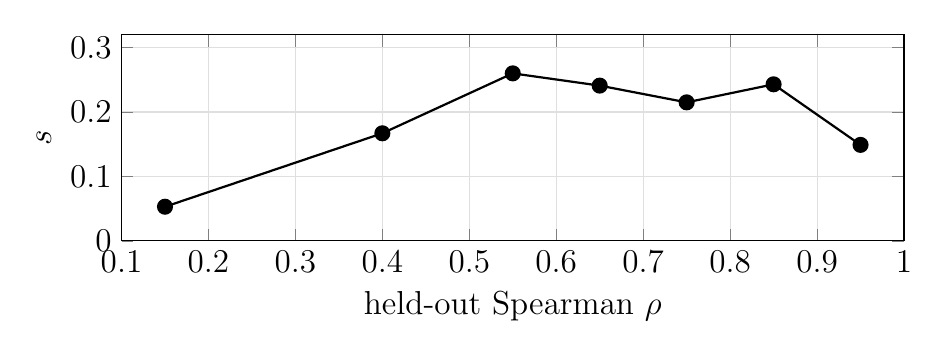
\begin{tikzpicture}
\begin{axis}[
  width=0.95\columnwidth, height=4.2cm,
  xlabel={held-out Spearman $\rho$},
  ylabel={$s$},
  label style={font=\large}, tick label style={font=\large},
  xmin=0.1, xmax=1.0, ymin=0, ymax=0.32,
  ytick={0,0.1,0.2,0.3}, grid=major, grid style={gray!25},
  mark size=2.5pt,
]
\addplot[thick, mark=*] coordinates {
 (0.15,0.053) (0.40,0.167) (0.55,0.260) (0.65,0.241)
 (0.75,0.215) (0.85,0.243) (0.95,0.149) };
\end{axis}
\end{tikzpicture}

\vskip 0.15in

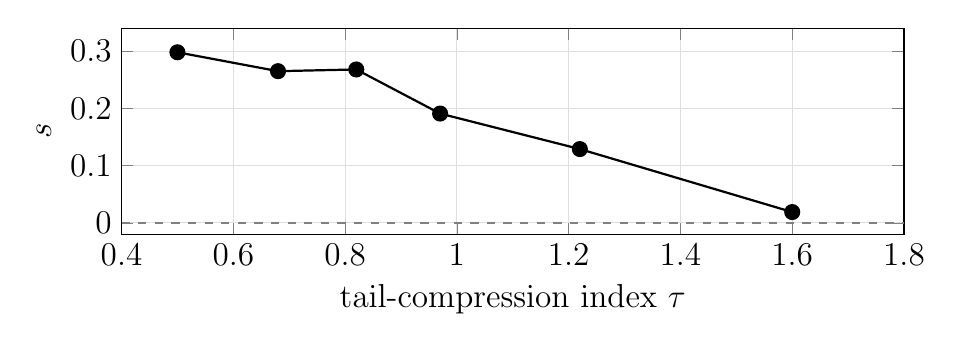
\begin{tikzpicture}
\begin{axis}[
  width=0.95\columnwidth, height=4.2cm,
  xlabel={tail-compression index $\tau$},
  ylabel={$s$},
  label style={font=\large}, tick label style={font=\large},
  xmin=0.4, xmax=1.8, ymin=-0.02, ymax=0.34,
  ytick={0,0.1,0.2,0.3}, grid=major, grid style={gray!25},
  mark size=2.5pt,
]
\addplot[thick, mark=*] coordinates {
 (0.50,0.298) (0.68,0.265) (0.82,0.268) (0.97,0.191)
 (1.22,0.129) (1.60,0.019) };
\addplot[dashed, gray, thick] coordinates {(0.4,0) (1.8,0)};
\end{axis}
\end{tikzpicture}
\end{center}
\caption{Normalized shortfall $s$ against surrogate accuracy (top) and against the
tail-compression index of \cref{eq:tau} (bottom). The shortfall is nearly flat in
accuracy above $\rho = 0.5$ but falls steadily as the upper tail of the fitness
distribution lengthens, approaching $0$ near $\tau = 1.6$. Points are medians over the
cells in each group of \cref{tab:byrho} and \cref{tab:tau}.}
\label{fig:main}
\end{figure}


\section{Experimental Setup}
\label{sec:setup}

\paragraph{Assays.}
We use the ProteinGym substitution benchmark, version $1.3$, which contains $217$ deep
mutational scanning assays \citep{notin2023proteingym}. Each assay provides a set of
single amino acid substitutions of one protein together with a measured fitness score.
We keep single substitutions, discard rows whose fitness is missing or not finite, and
require at least $200$ usable variants, which leaves $205$ assays for the selection
experiments. Assays with more than $20{,}000$ variants are subsampled to $20{,}000$ at a
fixed seed to bound computation. Every assay carries a coarse functional label in the
benchmark metadata, one of activity, binding, expression, organismal fitness, or
stability, which we use only for the breakdown in \cref{sec:results-class}.

\paragraph{Surrogate.}
The main surrogate is deliberately simple, because the claim concerns the form of the
reported score rather than any particular architecture. Each variant is described by additive features: a one-hot
indicator of the mutated position, one-hot indicators of the wild-type and mutant amino
acids, the BLOSUM62 score of the substitution \citep{henikoff1992amino}, and signed
differences in hydropathy \citep{kyte1982simple}, residue volume, and formal charge,
together with an indicator for gain or loss of proline. The features are additive by
construction so that the model generalizes to position and amino acid combinations it
has not seen. A one-hot encoding of the position and amino acid pair is degenerate on
single-mutant data, since each pair is measured once, and collapses to the intercept.
We fit ridge regression with the penalty chosen by cross-validation over $13$ values
spanning $10^{-2}$ to $10^{4}$. \Cref{sec:results-form} replaces it with a random
forest, gradient boosting, nearest neighbors, and ridge with a zero-shot language model
score appended, on identical splits.

\paragraph{Protocol.}
For each assay we draw a random split into a training fraction and a held-out
remainder, fit the surrogate on the training part, and score the held-out part. We use
training fractions of $0.1$, $0.3$, and $0.6$ to cover the data-poor regime that early
design rounds face, $5$ random seeds per fraction, and batch sizes $K \in \{10, 20,
50\}$. Predictions are never calibrated or tuned on held-out fitness. We report medians
across seeds and then across assays, and we compare selection rules with the Wilcoxon
signed-rank test on pairs matched by assay, training fraction, and batch size.

\paragraph{Correction rules.}
We test two families of correction, both restricted to information available at design
time. The first family rescales predictions. The rule \textsc{cal} fits a correction
$g(\yhat, \sigma)$ on a held-out slice of the training data, where $\sigma$ is the ridge
predictive standard deviation; \textsc{lcb} selects by $\yhat - c\sigma$ with $c$ chosen
on the same slice; \textsc{shrink} shrinks predictions toward the training median in
proportion to predictive variance. The second family changes which candidates are
chosen. Because ridge errors are correlated within a position, the rules
\textsc{cap}$m$ select greedily by prediction while allowing at most $m$ variants per
position, for $m \in \{1,2,3\}$, with \textsc{half} capping at $\max(1, K/10)$. Rules that alter only the forecast,
including isotonic regression, are fitted on the last $30\%$ of the training part,
which the surrogate does not see.

\section{Results}
\label{sec:results}

\subsection{Surrogates overpromise on real assays}
\label{sec:results-gap}

Across the $205$ assays, $93\%$ of assay and training-fraction combinations have a
positive shortfall. The median predicted gain is $1.091$ against a median realized gain
of $0.748$, so the median shortfall is $0.303$ and the median fraction of the ceiling
captured is $0.578$. The median held-out Spearman correlation is $0.691$, which is
comparable to what supervised models report on this benchmark.

\Cref{tab:byrho} breaks the normalized shortfall down by surrogate accuracy. Two
features stand out. The shortfall does not shrink as the surrogate improves: above
$\rho = 0.5$ it stays between $0.21$ and $0.26$ of the achievable gain. The overlap
between the selected batch and the true best batch stays small throughout, reaching
only $0.14$ for surrogates with $\rho$ between $0.8$ and $0.9$. A model whose held-out
correlation would place it near the top of a leaderboard still shares roughly one in
seven of its choices with the ideal batch.


\subsection{Tail compression predicts the shortfall and its sign}
\label{sec:results-tau}

\Cref{eq:main} attributes the shortfall to nonlinearity of the fitness quantile
transform, and \cref{eq:tau} summarizes the relevant nonlinearity in one number. Across
$607$ assay and training-fraction cells covering $204$ assays, the Spearman correlation
between $\tau$ and the normalized shortfall is $-0.470$ with $p = 9.9 \times 10^{-35}$.
Because $\tau$ and surrogate accuracy are themselves related, we also remove $\rho$
from both variables by linear regression and correlate the residuals, which gives
$-0.135$ with $p = 8 \times 10^{-4}$. The association is not a restatement of model
quality.

\Cref{tab:tau} and the lower panel of \cref{fig:main} show the relationship directly,
and the upper panel shows the contrast with accuracy. The shortfall falls monotonically as
the upper tail lengthens, from $0.298$ of the achievable gain in the most compressed
group to $0.019$ in the most extended one. The predicted reversal appears in the last
two rows: the proportion of cells where the surrogate underpromises rises from $0\%$ to
$42\%$.


\subsection{The pattern across assay types}
\label{sec:results-class}

Grouping assays by functional label gives the same picture in biological terms. Binding
assays are closest to Gaussian, with median $\tau = 1.011$ and the smallest shortfall at
$0.124$, while expression assays are the most compressed at $\tau = 0.843$ and the worst
affected at $0.325$ \mbox{(\cref{app:class})}.

Individual assays show the pattern more sharply. The SARS-CoV-2 spike receptor binding
domain has the most compressed tail in the benchmark, $\tau = 0.43$, and overstates the
achievable gain by $1.08$, which recalibration brings to $0.09$; human ACE2, with the
longest tail at $\tau = 1.86$, underpromises at $-0.06$. \Cref{tab:named} collects
these cases, including one instructive exception.


\subsection{Neither correction family recovers gain}
\label{sec:results-fix}

\Cref{cor:monotone} says that rescaling predictions cannot change the batch, so any
gain from the first family must come from its uncertainty term. \Cref{tab:fix}
confirms this: against a baseline that captures $0.452$ of the achievable gain,
\textsc{cal} is worse and the two uncertainty-aware rules move realized gain by at most
$0.002$. The second family does change the batch, spreading a batch of $10$ over $10$
positions where the baseline uses a median of $5$, and it still loses: every capping
rule reduces realized gain, by $0.014$ to $0.080$ of the achievable gain, winning at
most $23\%$ of comparisons. The baseline concentrates on those positions because that
is where the strong variants are.

Replacing greedy selection with an acquisition function does not change the picture
either. With the ridge posterior, upper confidence bounds at one and two standard
deviations, expected improvement, and Thompson sampling leave median gaps of $0.170$,
$0.171$, $0.171$, and $0.085$ against $0.169$ for greedy selection, and isotonic
recalibration removes most of the gap under each, winning on $74$ to $78\%$ of assays.
Greedy selection also captures the largest share of the achievable gain, $0.520$
against $0.370$ for Thompson sampling (\cref{app:acq}).


\subsection{Simulation confirms the theory and validates the statistic}
\label{sec:results-synth}

Real assays cannot test the theory's null, because no assay is exactly Gaussian, so we
sweep fitness shape directly. For a linear $G_{\!f}$, a saturating one, a bimodal one
that mimics the dead and functional clusters typical of deep mutational scanning, and
one with an extended upper tail, \cref{eq:main} truncated at $k = 8$ agrees with direct
simulation to within $1$ to $3\%$, and the linear shape reproduces \cref{cor:gaussian}
to simulation precision (\cref{app:fulltheory}). Sweeping shape continuously, with $y = \sinh(\operatorname{arcsinh}(z) /
\delta)$ for $\delta$ from $0.6$ to $3.0$ at accuracies $\rho$ from $0.5$ to $0.9$, \cref{fig:synth}
shows the gap crossing zero at $\tau = 1$, as \cref{cor:gaussian}
requires, running from $-0.125$ at $\tau = 1.59$ to $+0.129$ at $\tau = 0.75$, and
growing with accuracy from $0.049$ at $\rho = 0.5$ to $0.151$ at $\rho = 0.9$, which is
\cref{cor:saturation} in numbers. Across twelve unrelated distributions the rank
correlation between $\tau$ and the median gap is $-0.909$ at $p = 4.2 \times 10^{-5}$,
and under a hard upper ceiling the forecast overstates by $1.10$, more than the entire
achievable gain (\cref{app:shapes}).

The claim is prospective, since $\tau$ is available before any model is fit. Holding
out each of the $202$ real assays in turn and fitting a linear rule in $\log \tau$ and
$\rho$ on the rest predicts the held-out gap with mean absolute error $0.177$, against
$0.248$ for assuming no gap, which is what trusting the surrogate amounts to.
\Cref{app:shapes} reports the pooled and theory-anchored variants, neither of which
improves on it.


\subsection{Estimating the conditional mean repairs the forecast}
\label{sec:results-condmean}

\Cref{prop:tower} says the gap would vanish if the reported value were the conditional
mean, so the direct test is to estimate that conditional mean and see whether it does.
We fit three estimators of $m(\yhat)$ on a held-out slice of the training data only:
isotonic regression, a binned conditional mean, and Efron's Tweedie correction
\citep{efron2011tweedie}. Isotonic and binned are monotone, so by
\cref{cor:monotone} they leave the batch and the realized gain exactly as they were and
alter only the number attached to it.

\Cref{tab:condmean} reports the outcome over $202$ assays and $1509$ assay and budget
combinations. Isotonic regression cuts the mean absolute gap from $0.245$ to $0.100$
and the median gap from $0.166$ to $0.057$, improving on the reported score in $75.7\%$
of combinations. The binned estimator also improves on the mean absolute gap but
overshoots in the other direction, leaving a median gap of $-0.081$ and underpromising
in $83\%$ of combinations, because equal-count bins place too few points in the tail
that selection actually draws from. The Tweedie correction fails outright here, with a
mean absolute gap of $2.69$, since the empirical Bayes score is estimated from a
marginal density that is poorly resolved in the same tail. Split-conformal
recentering by the median calibration residual does not help either, at $0.293$, and a
$90\%$ conformal lower bound overcorrects to $0.512$ (\cref{tab:sota}).

\begin{table}[t]
\caption{Conditional-mean estimators against the reported score, over $202$ assays.
The gap is normalized by the achievable gain. Win rate and $p$ compare absolute gaps
against the reported score by a paired Wilcoxon signed-rank test.}
\label{tab:condmean}
\vskip 0.1in
\begin{center}
\begin{small}
\begin{tabular}{lrrrr}
\toprule
rule & median & mean $|\cdot|$ & win & $p$ \\
\midrule
reported score & $0.166$ & $0.245$ & n/a & n/a \\
isotonic       & $0.057$ & $0.100$ & $75.7\%$ & $10^{-120}$ \\
binned         & $-0.081$ & $0.177$ & $62.3\%$ & $10^{-21}$ \\
Tweedie        & $-1.270$ & $2.690$ & $1.6\%$ & $10^{-246}$ \\
\bottomrule
\end{tabular}
\end{small}
\end{center}
\vskip -0.1in
\end{table}

Tweedie need not be monotone, so it can also reorder candidates; used that way it
moves realized gain by a median of $-0.637$ and wins in $0.5\%$ of combinations, as
\cref{cor:monotone} leads one to expect of a rule that perturbs an ordering without
adding information.

\subsection{The correction under distribution shift}
\label{sec:results-shift}

Random splits leave the candidates exchangeable with the calibration slice, which is
the condition \cref{prop:tower} needs. Campaigns extrapolate, so we repeat the
experiment on four shifted splits of the same assays: positions held out, so that every
candidate mutates a site with no training measurement; mutant amino acids held out;
training confined to the lower $60\%$ of the fitness range; and training on single
substitutions with candidates carrying two or more, the combinatorial design case.
\Cref{tab:shift} reports the result.

The gap is largest where design is hardest. Candidates carrying multiple substitutions
overstate the achievable gain by a median of $0.741$, four times the value under random
splits, and candidates at unseen positions by $0.207$. Isotonic recalibration improves
the forecast in both, cutting the median absolute gap from $1.135$ to $0.947$ and from
$0.207$ to $0.136$, and winning on $64\%$ of assays in each. The other two splits
behave differently. With amino acids held out the reported score is already close to
unbiased and recalibration overshoots, raising the median absolute gap to $0.214$. With
training confined to the lower fitness range the rank accuracy of the surrogate
collapses to $-0.034$, the forecast underpromises, and every correction makes it worse. The pattern follows \cref{prop:tower} rather than
contradicting it, since a calibration slice identifies the conditional mean under the
distribution it is drawn from, which is the distribution the batch comes from in the
first two splits and not in the last two.

\begin{table}[t]
\caption{Median absolute gap under shifted splits, normalized by the achievable gain,
over $198$ assays and $56$ for the multiple substitution split. $\rho$ is the median
held-out rank accuracy.}
\label{tab:shift}
\vskip 0.1in
\begin{center}
\begin{small}
\begin{tabular}{lrrrr}
\toprule
split & $\rho$ & reported & linear & isotonic \\
\midrule
positions held out   & $\phantom{-}0.23$ & $0.207$ & $0.161$ & $0.136$ \\
amino acids held out & $\phantom{-}0.55$ & $0.164$ & $0.185$ & $0.214$ \\
low fitness only     & $-0.03$ & $0.151$ & $0.157$ & $0.261$ \\
singles to multiples & $\phantom{-}0.57$ & $1.135$ & $1.119$ & $0.947$ \\
\bottomrule
\end{tabular}
\end{small}
\end{center}
\vskip -0.1in
\end{table}

\subsection{The gap follows the form of the score, not its accuracy}
\label{sec:results-form}

If the gap were a weakness of ridge regression, a different surrogate would remove it.
We refit every split with a random forest, gradient boosting, and nearest neighbors
(\cref{tab:surrogates}). Ridge, boosting, and nearest neighbors overpromise in $86\%$,
$99.8\%$, and $90\%$ of combinations. The random forest does not: its median gap is
$-0.015$ and it overpromises in $17\%$. A forest prediction is an average of training
responses, which is an estimate of the conditional mean, and \cref{prop:tower} says
exactly that such a score carries no gap. Rank accuracy does not order the four:
boosting has the lowest accuracy, $\rho = 0.26$, and the largest gap, $0.455$, while
the forest sits in the middle at $\rho = 0.50$. A stronger surrogate does not help
either. Appending a zero-shot protein language model score to the ridge features
\citep{hsu2022learning}, using the ESM-2 \citep{lin2023evolutionary}, TranceptEVE,
SaProt, and ProSST scores distributed with ProteinGym, raises $\rho$ from $0.61$ to
between $0.68$ and $0.69$ and raises the median gap from $0.166$ to between $0.21$ and
$0.25$. Isotonic recalibration lowers the mean absolute gap of every surrogate, to
about $0.10$ for ridge and all four augmented models.

The closed form can also be confronted with the assays directly. Taking $G_{\!f}$ as
each assay's empirical quantile function and $\rho_\star$ from the observed $\rho$
through \cref{lem:rho}, with nothing fitted to the gaps, the model's gap correlates
with the observed gap at $r = 0.71$ over $1509$ combinations and matches its sign in
$79\%$; its captured gain correlates at $r = 0.86$. Iterating does not close the gap
either: over $3$ design rounds, each feeding its measured batch back into training, the
median gap falls from $0.222$ to $0.150$ while $89\%$ of assays still overpromise.

\subsection{The gap is not specific to protein fitness}
\label{sec:results-domains}

Everything above concerns one benchmark, so we repeated the experiment on four datasets
from three unrelated fields: superconductor critical temperature, small-molecule
solubility, two aquatic toxicity endpoints, and antimicrobial peptide activity. The
pipeline is unchanged; only the features differ, tabulated descriptors for the first
four and $2$-mer counts for the peptides. Across
$105$ dataset and budget combinations every domain overpromises, with median gaps from
$+0.01$ to $+1.28$, the peptides overstating by more than the entire achievable gain.
Isotonic recalibration cuts the pooled mean absolute gap from $0.385$ to $0.107$ at
$p = 2 \times 10^{-5}$ and improves four of the five, being worse only on
superconductors, the set with the highest surrogate accuracy and the smallest
uncorrected gap. Only the sign of the gap carries across domains, not its ordering by
$\tau$. \Cref{app:domains} gives the breakdown and the sources.

\section{Discussion}
\label{sec:discussion}

The results separate two questions that design practice usually treats as one: how good
the batch is, and how good the model says it is. \Cref{cor:monotone} makes the
separation exact, since a monotone rescaling moves the second without touching the
first, and the experiments bear it out: rescaling rules leave realized gain unchanged
and the one family that does change the batch makes it worse. Effort spent correcting
the forecast is well spent; effort spent reordering the library on the same surrogate
scores is not.

A surrogate with held-out correlation near $0.85$ still delivers about three quarters
of what it promises, so budgeting a campaign on the predicted gain overstates progress
per round by a margin that does not shrink as models improve and that \cref{eq:tau}
lets a team estimate from pilot measurements.

One feature of the data is not explained by \cref{eq:main} alone. The theory makes the
gap grow with accuracy for a fixed shape, while \cref{tab:byrho} is nearly flat above
$\rho = 0.5$, and \cref{sec:results-form} leaves real assays with roughly $0.08$ more
gap than the model near $\tau = 1$. Fitting the score on limited measurements is the
natural candidate, since the raw gap falls from $0.363$ to $0.232$ as the training
fraction rises from $0.1$ to $0.6$ while the theoretical term is unchanged.

\section{Conclusion}
\label{sec:conclusion}

Model-guided design selects candidates at the top of a predicted ranking, and the
predicted value of that batch overstates what it delivers by an amount set by the shape
of the fitness distribution and the form of the reported score rather than by the
accuracy of the model. The gap holds near a quarter of the achievable gain on $217$
deep mutational scanning assays, persists across surrogate families, acquisition rules,
and other domains, and is absent only for a surrogate whose output is already an
average. A statistic of the measured fitness values forecasts it before any
model is fit, and isotonic estimation of the conditional mean removes most of it
without changing the selected batch.

\section*{Impact Statement}

This work analyzes how model-guided design campaigns set expectations, using public
deep mutational scanning data. It introduces no new biological capability and proposes
no new molecules. The practical effect of adopting its conclusions is more conservative
forecasting of experimental rounds, which we expect to reduce wasted assay budget. We
see no specific societal risk that requires attention beyond the general considerations
that apply to protein engineering research.

\bibliographystyle{icml2027}
\bibliography{references}

\newpage
\appendix
\onecolumn

\section{Additional Theoretical Detail}
\label{app:theory}

\subsection{The Hermite reproducing identity}
\label{app:mehler}

The step used in the proof of \cref{thm:main} is that for $z \mid u \sim
\Normal(\rho_\star u, 1-\rho_\star^2)$,
\begin{equation}
\Exp\!\left[\He_k(z) \mid u\right] = \rho_\star^{\,k}\,\He_k(u).
\label{eq:mehler}
\end{equation}
This is the standard reproducing property of the Hermite polynomials under the
Ornstein-Uhlenbeck semigroup: the Hermite polynomials are eigenfunctions with
eigenvalues $\rho_\star^{\,k}$. Writing $z = \rho_\star u + \sqrt{1-\rho_\star^2}\,w$
with $w \sim \Normal(0,1)$ independent of $u$ and using the generating function
$\sum_k \He_k(x) t^k / k! = \exp(xt - t^2/2)$ gives \cref{eq:mehler} after matching
powers of $t$.

\subsection{Why the reference level cancels}
\label{app:base}

The gains in \cref{eq:predgain} and \cref{eq:realgain} both subtract the same reference
level $b$, so $S = \hat{G} - G$ does not depend on $b$. This is why
\cref{thm:main} can be stated without reference to how the baseline is chosen, and why
the empirical shortfall is insensitive to replacing the training median by the
wild-type fitness.

\subsection{Truncation of the Hermite series}
\label{app:trunc}

\Cref{tab:theory} evaluates \cref{eq:main} with the sum truncated at $k = 8$ and the
coefficients $c_k$ obtained by Gauss-Hermite quadrature with $200$ nodes. The remainder
is negligible for the saturating and extended-tail shapes but visible for the bimodal
shape at high accuracy, where $G_{\!f}$ has a sharp transition between the two modes and
the Hermite spectrum decays slowly. Increasing the truncation to $k = 12$ reduces the
discrepancy at $\rho_\star = 0.85$ from $0.026$ to $0.014$.

\section{Additional Empirical Detail}
\label{app:empirical}

\subsection{Breakdown by assay type}
\label{app:class}

\Cref{tab:class} gives the per-class medians summarized in \cref{sec:results-class}.

\begin{table}[ht]
\caption{Median tail-compression index, normalized shortfall, and surrogate accuracy by
functional assay class.}
\label{tab:class}
\vskip 0.1in
\begin{center}
\begin{small}
\begin{tabular}{lrrr}
\toprule
class & $\tau$ & $s$ & $\rho$ \\
\midrule
stability          & 0.726 & 0.235 & 0.788 \\
organismal fitness & 0.826 & 0.167 & 0.620 \\
activity           & 0.828 & 0.242 & 0.601 \\
expression         & 0.843 & 0.325 & 0.630 \\
binding            & 1.011 & 0.124 & 0.611 \\
\bottomrule
\end{tabular}
\end{small}
\end{center}
\end{table}

\subsection{Named assays across the tail range}
\label{app:named}

\Cref{tab:named} lists the assays discussed in \cref{sec:results-class}, ordered by
$\tau$. The gap is normalized by the achievable gain, so a value above one means the
forecast overstates by more than the entire gain available. Each row is the median over
training fractions, seeds and budgets for that assay.

\begin{table}[ht]
\caption{Gap before and after conditional-mean recalibration for named assays, ordered
by tail-compression index. The last two rows underpromise. GFP is the exception:
extended at $\tau = 1.12$ yet overstating by $0.86$, it is the smallest assay here and
the one the surrogate ranks worst, at $\rho = 0.12$, so its error reflects a failed fit
rather than tail shape.}
\label{tab:named}
\vskip 0.1in
\begin{center}
\begin{small}
\begin{tabular}{llrrrrr}
\toprule
protein & assay & $\tau$ & reported & isotonic & $\rho$ & variants \\
\midrule
spike RBD  & binding    & 0.43 & $+1.08$ & $+0.09$ & 0.72 & 3802 \\
ubiquitin  & fitness    & 0.50 & $+1.10$ & $+0.01$ & 0.68 & 1195 \\
DHFR       & fitness    & 0.72 & $+0.85$ & $+0.61$ & 0.58 & 2918 \\
PTEN       & activity   & 0.87 & $+0.36$ & $+0.13$ & 0.53 & 7260 \\
p53        & fitness    & 0.88 & $+0.12$ & $+0.06$ & 0.66 & 7467 \\
GFP        & expression & 1.12 & $+0.86$ & $+0.49$ & 0.12 & \phantom{0}433 \\
MPL        & fitness    & 1.13 & $-0.06$ & $+0.09$ & 0.51 & \phantom{0}562 \\
ACE2       & binding    & 1.86 & $-0.06$ & $+0.02$ & 0.56 & 2223 \\
\bottomrule
\end{tabular}
\end{small}
\end{center}
\vskip -0.1in
\end{table}

\subsection{Effect of training fraction}
\label{app:frac}

Raw shortfall falls with the amount of training data while the theoretical term of
\cref{eq:main} does not depend on it. At training fractions $0.1$, $0.3$, and $0.6$ the
median surrogate accuracy is $0.596$, $0.711$, and $0.733$, the median raw shortfall is
$0.363$, $0.317$, and $0.232$, and the median fraction of the ceiling captured is
$0.50$, $0.59$, and $0.63$. This is the trend referred to in \cref{sec:discussion}.

\subsection{Batch concentration}
\label{app:concentration}

The baseline concentrates its batch on few positions. At batch sizes $K = 10$, $20$,
and $50$ it uses a median of $5$, $9$, and $17$ distinct positions. The capping rules
raise this by construction, with \textsc{cap}$1$ reaching $K$ distinct positions by
definition, and \cref{tab:fix} reports the cost.

\begin{table}[ht]
\caption{Change in normalized realized gain against the top-$K$-by-prediction baseline,
paired by assay, training fraction, and batch size. The baseline captures $0.452$ of
the achievable gain for the rescaling family and $0.482$ for the batch family, which
use different numbers of usable pairs.}
\label{tab:fix}
\vskip 0.1in
\begin{center}
\begin{small}
\begin{tabular}{lrrr}
\toprule
rule & median $\Delta$ & wins & $p$ \\
\midrule
\textsc{cal}    & $-0.0022$ & 44.3\% & $3{\times}10^{-5}$ \\
\textsc{lcb}    & $+0.0000$ & 46.5\% & $2{\times}10^{-11}$ \\
\textsc{shrink} & $+0.0018$ & 56.0\% & $5{\times}10^{-14}$ \\
\midrule
\textsc{cap}1   & $-0.0797$ & 14.3\% & $10^{-203}$ \\
\textsc{cap}2   & $-0.0321$ & 20.1\% & $6{\times}10^{-156}$ \\
\textsc{cap}3   & $-0.0144$ & 23.2\% & $4{\times}10^{-114}$ \\
\textsc{half}   & $-0.0220$ & 21.0\% & $8{\times}10^{-137}$ \\
\bottomrule
\end{tabular}
\end{small}
\end{center}
\vskip -0.1in
\end{table}

\subsection{Shortfall by accuracy and by tail compression}
\label{app:strata}

\Cref{tab:byrho} and \cref{tab:tau} give the groupings plotted in \cref{fig:main}.

\begin{table}[ht]
\caption{Normalized shortfall $s$ and overlap between the selected batch and the true
best batch, by held-out Spearman correlation $\rho$. Overlap is the fraction of the
$20$ selected variants that are among the $20$ best.}
\label{tab:byrho}
\vskip 0.1in
\begin{center}
\begin{small}
\begin{tabular}{lrrr}
\toprule
$\rho$ & cells & $s$ & overlap \\
\midrule
$0.0$--$0.3$ & 20  & 0.053 & 0.01 \\
$0.3$--$0.5$ & 93  & 0.167 & 0.02 \\
$0.5$--$0.6$ & 81  & 0.260 & 0.07 \\
$0.6$--$0.7$ & 124 & 0.241 & 0.08 \\
$0.7$--$0.8$ & 169 & 0.215 & 0.12 \\
$0.8$--$0.9$ & 110 & 0.243 & 0.14 \\
$0.9$--$1.0$ & 10  & 0.149 & 0.23 \\
\bottomrule
\end{tabular}
\end{small}
\end{center}
\vskip -0.1in
\end{table}

\begin{table}[ht]
\caption{Normalized shortfall by tail-compression index $\tau$ from \cref{eq:tau}.
Lower $\tau$ means a more compressed upper tail. The last column gives the proportion
of cells with a negative shortfall, where the surrogate underpromises.}
\label{tab:tau}
\vskip 0.1in
\begin{center}
\begin{small}
\begin{tabular}{lrrrr}
\toprule
$\tau$ & cells & $s$ & $\rho$ & underpromise \\
\midrule
$<0.60$        & 115 & $+0.298$ & 0.78 & \phantom{0}3\% \\
$0.60$--$0.75$ & 158 & $+0.265$ & 0.75 & \phantom{0}2\% \\
$0.75$--$0.90$ & 113 & $+0.261$ & 0.67 & \phantom{0}0\% \\
$0.90$--$1.05$ & 81  & $+0.191$ & 0.63 & \phantom{0}4\% \\
$1.05$--$1.40$ & 81  & $+0.129$ & 0.62 & 12\% \\
$\ge 1.40$     & 59  & $+0.019$ & 0.54 & 42\% \\
\bottomrule
\end{tabular}
\end{small}
\end{center}
\vskip -0.1in
\end{table}

\subsection{Simulation protocol}
\label{app:sim-protocol}

Each cell draws $20{,}000$ candidates, holds out $30\%$ as a calibration slice, fits
the linear calibration and the conditional-mean estimators on that slice only, and
selects the top $K \in \{10, 20, 50\}$ by the reported score on the remainder. Gains
are taken relative to the median of the calibration slice, exactly as on real assays.
The shape sweep uses the sinh-arcsinh family with $\delta \in \{0.6, 0.8, 1.0, 1.3,
1.7, 2.2, 3.0\}$ and $20$ seeds per cell, giving $2{,}100$ cells. The heterogeneous
study replaces that family with twelve fixed distributions obtained by applying their
quantile functions to $\Phi(z)$, with $15$ seeds per cell.

\begin{figure}[ht]
\vskip 0.1in
\begin{center}
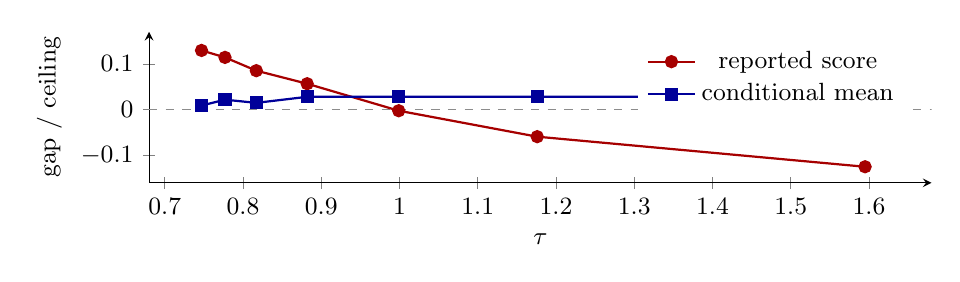
\begin{tikzpicture}
\begin{axis}[
  width=0.95\columnwidth, height=3.5cm,
  xlabel={$\tau$}, ylabel={gap / ceiling},
  label style={font=\small}, tick label style={font=\small},
  legend style={font=\small, draw=none, at={(0.97,0.95)}, anchor=north east},
  axis lines=left, xmin=0.68, xmax=1.68, ymin=-0.16, ymax=0.17,
]
\addplot[black!45, dashed, forget plot] coordinates {(0.68,0) (1.68,0)};
\addplot[mark=*, thick, color=red!65!black] coordinates {
  (0.747,0.1292) (0.777,0.1140) (0.817,0.0850) (0.882,0.0565)
  (0.999,-0.0025) (1.176,-0.0592) (1.595,-0.1249)};
\addlegendentry{reported score}
\addplot[mark=square*, thick, color=blue!60!black] coordinates {
  (0.747,0.0088) (0.777,0.0216) (0.817,0.0147) (0.882,0.0279)
  (0.999,0.0281) (1.176,0.0279) (1.595,0.0286)};
\addlegendentry{conditional mean}
\end{axis}
\end{tikzpicture}
\end{center}
\caption{Median gap against the tail-compression index over the shape sweep. The
reported score crosses zero at $\tau = 1$ and reverses sign, while the estimated
conditional mean stays near zero throughout.}
\label{fig:synth}
\vskip -0.15in
\end{figure}

\subsection{Tail-compression index across unrelated distributions}
\label{app:shapes}

\Cref{tab:shapes} gives the per-distribution medians behind the rank correlation of
$-0.909$ quoted in \cref{sec:results-synth}. The Gaussian row is the control and sits
at $-0.008$, and the truncated row is the saturating case. Holding out each distribution
in turn, a linear rule in $\log \tau$ constrained to vanish at $\tau = 1$ predicts the
held-out gap better than assuming no gap on $10$ of the $12$, at $p = 0.005$. That
constraint does not help on real assays: against the leave-one-assay-out error of
$0.177$ for the free rule quoted in \cref{sec:results-synth}, a pooled mean gives
$0.187$ and the rule anchored to vanish at $\tau = 1$ gives $0.218$, because real
assays retain a gap at $\tau = 1$ that the idealized model does not contain.

\begin{table}[ht]
\caption{Median tail-compression index and median normalized gap for the reported
score and for isotonic recalibration, by distribution.}
\label{tab:shapes}
\vskip 0.1in
\begin{center}
\begin{small}
\begin{tabular}{lrrr}
\toprule
distribution & $\tau$ & reported & isotonic \\
\midrule
truncated upper & $0.343$ & $1.101$ & $0.026$ \\
inverse square root & $0.532$ & $0.271$ & $0.051$ \\
uniform & $0.567$ & $0.351$ & $0.039$ \\
beta$(5,2)$ & $0.665$ & $0.427$ & $0.038$ \\
bimodal & $0.995$ & $0.436$ & $0.082$ \\
Gaussian & $0.998$ & $-0.008$ & $0.072$ \\
beta$(2,5)$ & $1.018$ & $-0.079$ & $0.067$ \\
logistic & $1.211$ & $-0.085$ & $0.077$ \\
gamma$(2)$ & $1.412$ & $-0.205$ & $0.085$ \\
exponential & $1.629$ & $-0.266$ & $0.085$ \\
Student $t_3$ & $1.710$ & $-0.187$ & $0.115$ \\
lognormal & $2.216$ & $-0.277$ & $0.095$ \\
\bottomrule
\end{tabular}
\end{small}
\end{center}
\vskip -0.1in
\end{table}

\subsection{Shrinking the conditional-mean estimator}
\label{app:shrink}

Isotonic regression is nonparametric and therefore noisy when the score carries little
signal: in simulation it loses to the linear calibration below $\rho = 0.7$, with mean
absolute gap $0.080$ against $0.049$ at $\rho = 0.5$. A convex weight $w$ between the
linear and isotonic fits, chosen by five-fold cross-validation inside the calibration
slice, removes that failure. Because a convex combination of two increasing maps is
increasing, the ranking and therefore the batch are unchanged, which we verified on
every cell.

The weight must be chosen on the region that is actually selected. Minimizing overall
squared error shrinks too far on severely misspecified shapes, giving $0.178$ against
isotonic's $0.026$ under a hard ceiling. Restricting the cross-validation objective to
the top $1\%$ of scores fixes this and yields the lowest mean absolute gap of any rule
we tried, $0.066$ against $0.069$ for isotonic and $0.320$ for the reported score, with
a median gap of zero to four decimal places. The learned weight is interpretable,
rising from $0.24$ under Gaussian fitness, where \cref{cor:gaussian} says there is
nothing to correct, to $1.00$ under a hard ceiling. Against isotonic the difference is
not significant cell by cell ($p = 0.22$); the gain is in avoiding large errors rather
than in winning more often.

The advantage does not carry over to real assays. On the same splits as
\cref{sec:results-condmean}, where calibration slices hold a few hundred points and the
tail window must widen to the top $20\%$ of scores, the tail-weighted variant reaches a
mean absolute gap of $0.125$ against $0.100$ for isotonic regression and $0.245$ for the
reported score, and isotonic regression is the better of the two in $71.7\%$ of
combinations ($p = 10^{-35}$). The learned weight averages $0.50$, so the blend
retains half of the linear calibration's error where the full correction was needed.
Plain isotonic regression is therefore the estimator we recommend.

\subsection{Datasets outside protein fitness}
\label{app:domains}

\Cref{tab:domains} reports the four additional datasets of
\cref{sec:results-domains}, each the median over training fractions, seeds and budgets.
Superconductor critical temperatures come from the UCI superconductivity set, solubility
from the Delaney set using its six physical descriptors only, with its precomputed
solubility prediction excluded so that no model output enters the features, the two
toxicity endpoints from the UCI QSAR sets, and peptide activity from GRAMPA
\citep{witten2019deep}, restricted to \emph{E. coli} and reduced to a median log
concentration per sequence.

\begin{table}[ht]
\caption{Gap before and after conditional-mean recalibration outside protein fitness.
Every median gap is positive. Isotonic regression improves all but the superconductor
set, which has the highest surrogate accuracy and the smallest uncorrected gap.}
\label{tab:domains}
\vskip 0.1in
\begin{center}
\begin{small}
\begin{tabular}{lrrrrr}
\toprule
dataset & cells & $\tau$ & reported & isotonic & $\rho$ \\
\midrule
superconductors & 25 & 0.68 & $0.097$ & $0.120$ & 0.84 \\
solubility      & 20 & 0.89 & $0.156$ & $0.104$ & 0.83 \\
peptides        & 25 & 0.97 & $1.270$ & $0.138$ & 0.40 \\
aquatic toxicity & 15 & 1.22 & $0.114$ & $0.095$ & 0.67 \\
fish toxicity   & 20 & 1.32 & $0.071$ & $0.066$ & 0.78 \\
\midrule
pooled          & 105 & n/a & $0.385$ & $0.107$ & n/a \\
\bottomrule
\end{tabular}
\end{small}
\end{center}
\vskip -0.1in
\end{table}

\subsection{Other surrogates, design rounds, and the closed form on real assays}
\label{app:form}

\Cref{tab:surrogates} gives the surrogate comparison of \cref{sec:results-form} on
$195$ assays, with identical splits for every model and $4368$ combinations each. The
size of the calibration slice matters little: isotonic mean absolute gaps are $0.145$,
$0.142$, and $0.137$ at $20\%$, $30\%$, and $45\%$ of the training data.
\Cref{tab:rounds} gives the three design rounds, with a budget of $20$ per round, and
\cref{tab:closedform} compares the closed-form gap with the observed gap by tail
stratum. The model reproduces the decline with $\tau$ and sits $0.07$ to $0.09$ below
the observations for $\tau$ above $0.75$.

\begin{table}[ht]
\caption{The gap under four surrogates on identical splits. The random forest, whose
prediction is an average of training responses, is the only one without a gap.}
\label{tab:surrogates}
\vskip 0.1in
\begin{center}
\begin{small}
\begin{tabular}{lrrrrr}
\toprule
surrogate & $\rho$ & median & mean $|\cdot|$ & isotonic & over \\
\midrule
ridge             & 0.59 & $+0.164$ & 0.254 & 0.111 & 86.4\% \\
random forest     & 0.50 & $-0.015$ & 0.164 & 0.103 & 16.7\% \\
gradient boosting & 0.26 & $+0.455$ & 0.515 & 0.186 & 99.8\% \\
nearest neighbors & 0.31 & $+0.158$ & 0.196 & 0.160 & 89.6\% \\
\bottomrule
\end{tabular}
\end{small}
\end{center}
\vskip -0.1in
\end{table}

\begin{table}[ht]
\caption{Surrogates built on zero-shot protein language model scores, alone after a
fitted linear map or appended to the ridge features, and split-conformal forecast rules
for the ridge surrogate. Mean absolute gap before and after isotonic recalibration.}
\label{tab:sota}
\vskip 0.1in
\begin{center}
\begin{small}
\begin{tabular}{lrrrr}
\toprule
surrogate & $\rho$ & median & mean $|\cdot|$ & isotonic \\
\midrule
ridge               & 0.61 & $0.166$ & 0.245 & 0.100 \\
ridge + ESM-2       & 0.68 & $0.214$ & 0.330 & 0.093 \\
ridge + ProSST      & 0.69 & $0.216$ & 0.294 & 0.103 \\
ridge + SaProt      & 0.68 & $0.210$ & 0.337 & 0.098 \\
ridge + TranceptEVE & 0.69 & $0.247$ & 0.367 & 0.090 \\
ESM-2 alone         & 0.49 & $0.292$ & 0.335 & 0.167 \\
ProSST alone        & 0.52 & $0.263$ & 0.458 & 0.259 \\
SaProt alone        & 0.50 & $0.235$ & 0.331 & 0.155 \\
TranceptEVE alone   & 0.47 & $0.181$ & 0.333 & 0.114 \\
\midrule
\multicolumn{5}{l}{forecast rule, ridge surrogate} \\
conformal recentering   & & $0.181$ & 0.293 & \\
tail-restricted recentering & & $0.129$ & 0.219 & \\
conformal lower bound   & & $-0.387$ & 0.512 & \\
\bottomrule
\end{tabular}
\end{small}
\end{center}
\vskip -0.1in
\end{table}

\begin{table}[ht]
\caption{The gap over successive design rounds, each adding its measured batch to the
training data.}
\label{tab:rounds}
\vskip 0.1in
\begin{center}
\begin{small}
\begin{tabular}{rrrrrr}
\toprule
round & training & $\rho$ & median & isotonic & over \\
\midrule
1 & 154 & 0.46 & $+0.222$ & 0.156 & 87.9\% \\
2 & 174 & 0.47 & $+0.181$ & 0.093 & 89.9\% \\
3 & 194 & 0.50 & $+0.150$ & 0.075 & 88.9\% \\
\bottomrule
\end{tabular}
\end{small}
\end{center}
\vskip -0.1in
\end{table}

\begin{table}[ht]
\caption{Median gap observed on real assays and predicted by the closed-form model with
no fitted parameters, by tail-compression stratum.}
\label{tab:closedform}
\vskip 0.1in
\begin{center}
\begin{small}
\begin{tabular}{lrrr}
\toprule
$\tau$ & cells & observed & model \\
\midrule
$<0.60$        & 204 & $0.208$ & $0.274$ \\
$0.60$--$0.75$ & 357 & $0.233$ & $0.293$ \\
$0.75$--$0.90$ & 285 & $0.223$ & $0.165$ \\
$0.90$--$1.05$ & 234 & $0.159$ & $0.092$ \\
$1.05$--$1.40$ & 264 & $0.099$ & $0.006$ \\
$\ge 1.40$     & 165 & $0.021$ & $-0.021$ \\
\bottomrule
\end{tabular}
\end{small}
\end{center}
\vskip -0.1in
\end{table}

\subsection{Acquisition rules and shifted splits}
\label{app:acq}

\Cref{tab:acq} gives the acquisition comparison of \cref{sec:results-fix} over $202$
assays on identical splits, with the ridge posterior supplying the predictive standard
deviation. Thompson sampling selects a less concentrated batch, which both lowers the
share of the achievable gain it captures and reduces the gap, as \cref{thm:main}
implies for a selection that reaches less far into the tail.

For the shifted splits of \cref{sec:results-shift}, the positions and amino acids are
divided in half at random and resampled over $5$ seeds, the low fitness split trains on
the lowest $60\%$ of measured variants, and the multiple substitution split trains on
every single substitution and selects among variants carrying two or more, with
features summed over the constituent substitutions. Cross-fitted and tail-weighted
isotonic behave like plain isotonic throughout, with median absolute gaps of $0.143$
and $0.134$ for positions held out and $0.959$ and $0.951$ for multiple substitutions.

\begin{table}[ht]
\caption{Median gap and share of the achievable gain captured, by acquisition rule.
The win rate compares the absolute gap of isotonic recalibration against the reported
score at assay level.}
\label{tab:acq}
\vskip 0.1in
\begin{center}
\begin{small}
\begin{tabular}{lrrrr}
\toprule
rule & reported & isotonic & captured & win \\
\midrule
greedy               & $0.169$ & $0.062$ & $0.520$ & $77\%$ \\
UCB, $1\sigma$       & $0.170$ & $0.060$ & $0.512$ & $78\%$ \\
UCB, $2\sigma$       & $0.171$ & $0.062$ & $0.497$ & $75\%$ \\
expected improvement & $0.171$ & $0.066$ & $0.495$ & $74\%$ \\
Thompson sampling    & $0.085$ & $0.027$ & $0.370$ & $76\%$ \\
\bottomrule
\end{tabular}
\end{small}
\end{center}
\vskip -0.1in
\end{table}

\subsection{Full theory and simulation comparison}
\label{app:fulltheory}

\Cref{tab:theory} reports a subset of accuracies. Across $\rho_\star \in \{0.3, 0.6,
0.85, 1.0\}$ and the four fitness shapes, the mean absolute difference between
\cref{eq:main} and simulation is $0.013$ in fitness units, with the largest single
discrepancy $0.098$ at $\rho_\star = 1.0$ for the bimodal shape, attributable to series
truncation as described in \cref{app:trunc}.

\begin{table}[ht]
\caption{Shortfall predicted by \cref{eq:main} against simulation, for four fitness
shapes and four accuracies. Linear fitness gives zero at every accuracy, and the
extended tail gives a negative shortfall, meaning the surrogate underpromises.}
\label{tab:theory}
\vskip 0.1in
\begin{center}
\begin{small}
\begin{tabular}{lcccc}
\toprule
$G_{\!f}$ & $\rho_\star$ & theory & simulation \\
\midrule
extended tail & 0.60 & $-0.393$ & $-0.399$ \\
extended tail & 0.85 & $-0.910$ & $-0.906$ \\
linear        & 0.60 & $\phantom{-}0.000$ & $-0.001$ \\
linear        & 0.85 & $\phantom{-}0.000$ & $\phantom{-}0.001$ \\
bimodal       & 0.60 & $\phantom{-}0.112$ & $\phantom{-}0.115$ \\
bimodal       & 0.85 & $\phantom{-}0.360$ & $\phantom{-}0.334$ \\
saturating    & 0.60 & $\phantom{-}0.273$ & $\phantom{-}0.272$ \\
saturating    & 0.85 & $\phantom{-}0.594$ & $\phantom{-}0.590$ \\
\bottomrule
\end{tabular}
\end{small}
\end{center}
\vskip -0.1in
\end{table}


\end{document}
